\documentclass{beamer}
%
% Choose how your presentation looks.
%
% For more themes, color themes and font themes, see:
% http://deic.uab.es/~iblanes/beamer_gallery/index_by_theme.html
%
\mode<presentation>
{
  \usetheme{default}      % or try Darmstadt, Madrid, Warsaw, ...
  \usecolortheme{default} % or try albatross, beaver, crane, ...
  \usefonttheme{default}  % or try serif, structurebold, ...
  \setbeamertemplate{navigation symbols}{}
  \setbeamertemplate{caption}[numbered]
} 


\usepackage[english,russian]{babel}
\usepackage[utf8x]{inputenc}

\title[Your Short Title]{Обзор статьи: "Jackson’s Pseudo Preemptive Schedule for the $Pm/r_i , q_i/C_{max}$ scheduling problem"}
\institute{ }
\author{}
\date{ }

\begin{document}

\begin{frame}
  \titlepage
\end{frame}

\section{Доклад}


% 
%
%
\begin{frame}{$Pm/r_i , q_i/C_{max}$ scheduling problem}
    $n$- число операций,\\
    $m$- число параллельных идентичных процессоров,\\
    $r_i$- release date or head,\\
    $q_i$- latency duration or tail,\\
    $C_{max}$- длина расписания
    
    
\end{frame}

%  Первый функционал мы будем называть функционалом Хаусдорфа пространства $(X, \Omega, h)$;
% он является внешней мерой на $X$ 
% 
% Второй же функционал был определен в несколько меньшей общности в статье одного из авторов.
% Без дополнительных предположений о размерностном пространстве он не является внешней мерой;
% поэтому мы будем называть его функционалом Хаусдорфа-Лебега.
\begin{frame}{Jackson’s Pseudo Preemptive Schedule
}
   The algorithm:\\
t =0\\
S = ∅; A = ∅ (S denotes the set of completed operations at the current time t, A the
set of available operations)\\
Do Until S = I\\
Update A and S\\ If A ≠ ∅ then\\
compute the current schedule block B, and the associated operation rates compute the next decision time $\theta$\\
t = $t + \theta$ ($t + \theta$ is the time where the current schedule block B has to be modified)\\
Else\\
compute the first time t where A ≠ ∅\\
Endif\\ Enddo
    
\end{frame}


\begin{frame}{Пример}
    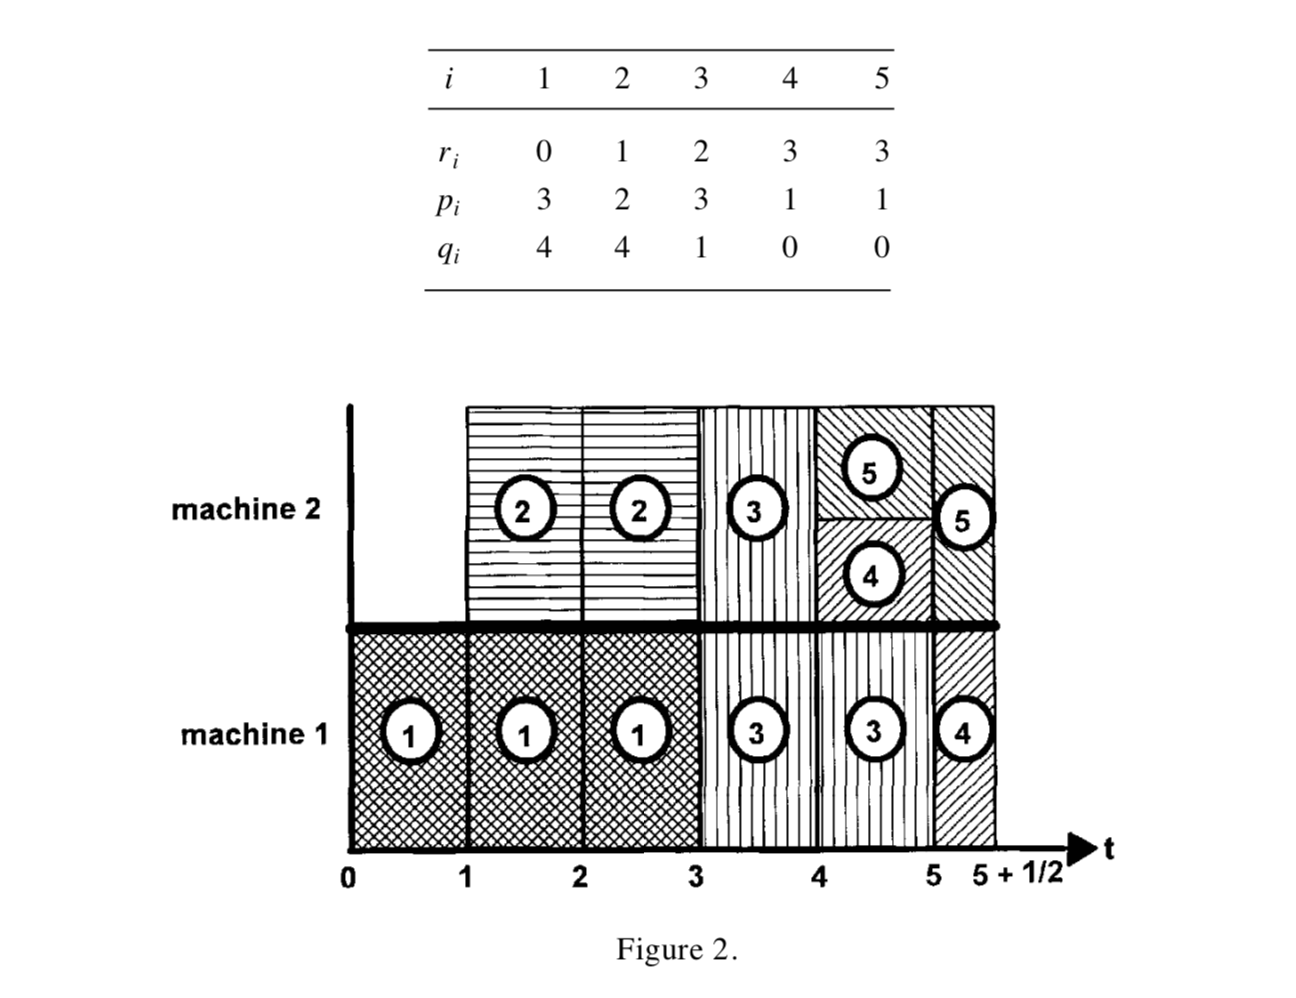
\includegraphics[scale=0.5]{universe}  
\end{frame}


\begin{frame}{Вычисление текущего блока}
    \textbf{Предположение 1} 
      
    
\end{frame}

\begin{frame}{Вычисление $\theta$(decision time)}
      События которые могут изменить текущий блок принадлежат одному из типов:
      \begin{enumerate}
        \item E1 Операция становится доступной.
        \item E2 Операция закончена.
        \item E3 Доступная операция начинает выполнятся.
        \item E4 Полностью доступная операция становится частично доступной.
        \item E5 Частично доступная операция становится полностью доступной.

    \end{enumerate}
\end{frame}

\begin{frame}{Вычисление $\theta$(decision time)}
    \textbf{Предположение 2}\\
      $\theta = min(\theta_1, \theta_2, \theta_3, \theta_4, \theta_5)$, где $t + \theta_k$, $k \in 1:5$, первый раз когда событие типа $E_k$ может возникнуть и
$\theta_1 = {\underset{j \in A}{min}}$ $r_j − t$,
$\theta_2 = {\underset{j \in B}{min}}\frac{a_j(t)}{\alpha_j(t)}$,
$\theta_3 = {\underset{j \in B}{min}}\frac{c_j(t)-c_{max}}{\alpha_j(t)}$,
$\theta_4 = {\underset{j \in T}{min}}\frac{t-(r_j+p_j-a_j(t))}{\alpha_T-1}$,
$\theta_5 = {\underset{j \in P}{min}}\frac{c_j(t)-c_T}{1-\alpha_T}$, где $c_{max} = {\underset{i \in A-B}{max}}$, и $c_T$ максимальный полный хвост операций из T.
    
\end{frame}


% 
% 
% 
\begin{frame}{Свойства JPPS}
 \textbf{Предположение 3} \\
\begin{enumerate}
      \item Максимальное число событий типов E1, E2, и E3  O(n).
      \item Максимальное число событий типов E4 и E5  O(nm).\\
\end{enumerate}
$\\$
    \textbf{Теорема 1} \\
    Максимальное число блоков в JPPS  O(nm).
\end{frame}

% 
% 
% 
\begin{frame}{Теорема 2}
    \textbf{Теорема 2.}
    
    $$
    C (JPPS) =
    max\{
        \underset{i \in I}{max} (r_i p_i + q_i),
        \underset{J \subseteq I, |J| \geq m}{max} G' (J)
        \}
    $$.
\end{frame}

% 
% 
% 
\begin{frame}{Вспомогательные утверждения}
    \textbf{Лемма 1.}
    
    $$
    C (JPPS) \geq
        \underset{J \subseteq I}{max} G' (J)
    $$.
\end{frame}

% В этом разделе мы предлагаем алгоритм времени
% со сложность O (n log n + nm log m) для вычисления 
% промежуточного периода C (JPPS) для JPPS. 
% Мы представляем структуры данных, которые позволяют
% эффективное выполнение двух основных этапов этой процедуры:
%вычислениетекущего блока расписания и 
% следующего времени принятия решения.
\begin{frame}{O(n log n + nm log m)}
    \textbf{Теорема 3.}
    
    C(JSSP) может быть вычесленно за O(n log n + nm log m). 
    Кроме того, определение множества $J_0$ из Теоремы 2, вычисляется с той же сложностью (если оно существует).
    \newline
    
    \textbf{Теорема 4.}
    
    Верхняя оценка сложности построения JPPS это O($n^2 + nm^2$).
\end{frame}

% 
% 
% 
\section{Литература}

\begin{frame}{Литература}
    \begin{enumerate}
    	\item 
    	   J. Carlier and E. Pinson. Jackson’s Pseudo Preemptive Schedule for the $Pm/r_i , q_i/C_{max}$ scheduling problem. Annals of Operations Research 83(1998)41–58.
    \end{enumerate}
\end{frame}


\end{document}

